\documentclass[]{article}
\usepackage{lmodern}
\usepackage{amssymb,amsmath}
\usepackage{ifxetex,ifluatex}
\usepackage{fixltx2e} % provides \textsubscript
\ifnum 0\ifxetex 1\fi\ifluatex 1\fi=0 % if pdftex
  \usepackage[T1]{fontenc}
  \usepackage[utf8]{inputenc}
\else % if luatex or xelatex
  \ifxetex
    \usepackage{mathspec}
  \else
    \usepackage{fontspec}
  \fi
  \defaultfontfeatures{Ligatures=TeX,Scale=MatchLowercase}
\fi
% use upquote if available, for straight quotes in verbatim environments
\IfFileExists{upquote.sty}{\usepackage{upquote}}{}
% use microtype if available
\IfFileExists{microtype.sty}{%
\usepackage{microtype}
\UseMicrotypeSet[protrusion]{basicmath} % disable protrusion for tt fonts
}{}
\usepackage[margin=1in]{geometry}
\usepackage{hyperref}
\hypersetup{unicode=true,
            pdftitle={ESM206\_Assignment4},
            pdfauthor={Geoffrey Cook},
            pdfborder={0 0 0},
            breaklinks=true}
\urlstyle{same}  % don't use monospace font for urls
\usepackage{graphicx,grffile}
\makeatletter
\def\maxwidth{\ifdim\Gin@nat@width>\linewidth\linewidth\else\Gin@nat@width\fi}
\def\maxheight{\ifdim\Gin@nat@height>\textheight\textheight\else\Gin@nat@height\fi}
\makeatother
% Scale images if necessary, so that they will not overflow the page
% margins by default, and it is still possible to overwrite the defaults
% using explicit options in \includegraphics[width, height, ...]{}
\setkeys{Gin}{width=\maxwidth,height=\maxheight,keepaspectratio}
\IfFileExists{parskip.sty}{%
\usepackage{parskip}
}{% else
\setlength{\parindent}{0pt}
\setlength{\parskip}{6pt plus 2pt minus 1pt}
}
\setlength{\emergencystretch}{3em}  % prevent overfull lines
\providecommand{\tightlist}{%
  \setlength{\itemsep}{0pt}\setlength{\parskip}{0pt}}
\setcounter{secnumdepth}{0}
% Redefines (sub)paragraphs to behave more like sections
\ifx\paragraph\undefined\else
\let\oldparagraph\paragraph
\renewcommand{\paragraph}[1]{\oldparagraph{#1}\mbox{}}
\fi
\ifx\subparagraph\undefined\else
\let\oldsubparagraph\subparagraph
\renewcommand{\subparagraph}[1]{\oldsubparagraph{#1}\mbox{}}
\fi

%%% Use protect on footnotes to avoid problems with footnotes in titles
\let\rmarkdownfootnote\footnote%
\def\footnote{\protect\rmarkdownfootnote}

%%% Change title format to be more compact
\usepackage{titling}

% Create subtitle command for use in maketitle
\newcommand{\subtitle}[1]{
  \posttitle{
    \begin{center}\large#1\end{center}
    }
}

\setlength{\droptitle}{-2em}

  \title{ESM206\_Assignment4}
    \pretitle{\vspace{\droptitle}\centering\huge}
  \posttitle{\par}
    \author{Geoffrey Cook}
    \preauthor{\centering\large\emph}
  \postauthor{\par}
      \predate{\centering\large\emph}
  \postdate{\par}
    \date{11/13/2018}

\usepackage{booktabs}
\usepackage{longtable}
\usepackage{array}
\usepackage{multirow}
\usepackage[table]{xcolor}
\usepackage{wrapfig}
\usepackage{float}
\usepackage{colortbl}
\usepackage{pdflscape}
\usepackage{tabu}
\usepackage{threeparttable}
\usepackage{threeparttablex}
\usepackage[normalem]{ulem}
\usepackage{makecell}

\begin{document}
\maketitle

\subsection{Introduction}\label{introduction}

The California Spiny Lobster, Panulirus interruptus, is a marine
crustacean found along the coast from Point Conception in Santa Barbara
County to the US-Mexican border.\(^3\) Lobster fishing in this area has
a deep history and continues today. The spiny lobster is the only
invertebrate in California that is subject to both a significant
recreational and commercial fishery.\(^1\) In an effort to study and
understand the impacts of human activities on coastal ecosystems, Santa
Barbara Coastal Long Term Ecological Research conducted a study on the
California Spiny Lobster.\(^6\) Data including lobster abundance and
size was gathered at various giant kelp forest ecosystems sites along
the southern California coast.

Lobster abundance is simply measured as a count. In the Long Term
Ecological Research study, the abundance of lobsters of different sizes
was collected. Abundance can be affected by a multitude of factors,
including predation. The spiny lobster is prey to various marine species
including giant sea bass, California sheephead, cabezon, horn shark,
leopard shark, octopus and sea otters.\(^2\) Humans are also predators
and have been for hundreds of years. Documented lobster fishing in the
region between Santa Barbara County and the US-Mexican border has been
recorded since the late 1800s.\(^1\) By the 1900s, lobster counts were
decreasing significantly. Preliminary measures were enacted to limit
rapid decline in population due to human forces. These regulations
included seasonal fishing and size limits for catch.\(^1\) Size
limitations are still currently enforced.

Lobster size is an important ecological factor. The body length of the
lobster larva is about 1.4 mm at at the first stage of its development
and about 29 mm at the final larva development stage.\(^7\) This
measurement is taken along the length of the body shell, or carapace,
from the edge of the eye socket to the rear edge of the carapace.\(^2\)
Once a juvenile, carapace length increases about 3.1 mm after each molt
(shedding of the old shell).\(^7\) Juveniles reach approximately 24 mm
after 1 year and 44 mm after 2 years. A length of 82.6 mm is expected
after approximately 7 to 10 years.\(^7\) This 82.6 mm value is of
importance because this has been established as the legal limit for
lobster catch. Once lobsters have reached this size, fishermen can keep
the lobster instead of returning it to the ocean. The minimum size limit
was established with the intent to allow each lobster to reproduce at
least once before it is captured.\(^2\) In the Santa Barbara Coastal
Long Term Ecological Research study, a range of carapace sizes were
observed in various sites.\(^5\)

Multiple sites were defined and observed in the Santa Barbara Long Term
Ecological Research study involving the California Spiny Lobster. Our
analysis in this research paper focuses on five of the sites: Arroyo
Quemado (AQUE), Naples Reef (NAPL), Mohawk Reef (MOHK), Isla Vista
(IVEE), Carpinteria (CARP). Lobster size and abundance was observed and
recorded at each of the sites from 2012-08-20 to 2017-08-25 (5). Two of
the sites, Naples and Isla Vista, are located in the California Fish and
Game Network of Marine Protected Areas (MPA).\(^5\) MPAs are defined
marine or estuarine areas designed to protect or conserve marine life
and habitat. According to NOAA's MPA inventory database, Naples' primary
conservation focus is natural heritage. Commercial and recreational
fishing are restricted year round. The Isla Vista site is listed as
Campus Point State Marine Conservation Area in the NOAA database. The
protection focus is the ecosystem, and commercial and recreational
fishing are also restricted year round.\(^4\) Major revisions and
additions to Southern California MPAs went into effect in state waters
on January 1, 2012. Both Naples and Isla Vista were established as MPAs
on this date.

\subsection{Data and Methods}\label{data-and-methods}

Data was provided from the SBC LTER: Reef: Abundance, size and fishing
effort for California Spiny Lobster from years 2012 to 2017. Fishing
pressure was determined through counted number of fishing trap floats
recorded in five locations(Isla Vista, Naples, Arroyo Quemado, Mohawk
Reef, and Carpinteria) two of which are designated Marine Protected
Areas (Isla Vista and Naples). Observations were collected every 2 to 4
weeks during lobster fishing season (October to March). Abundance and
size data was recorded annually by divers in the months immediately
prior to the start of lobster fishing season.

\begin{figure}
\centering
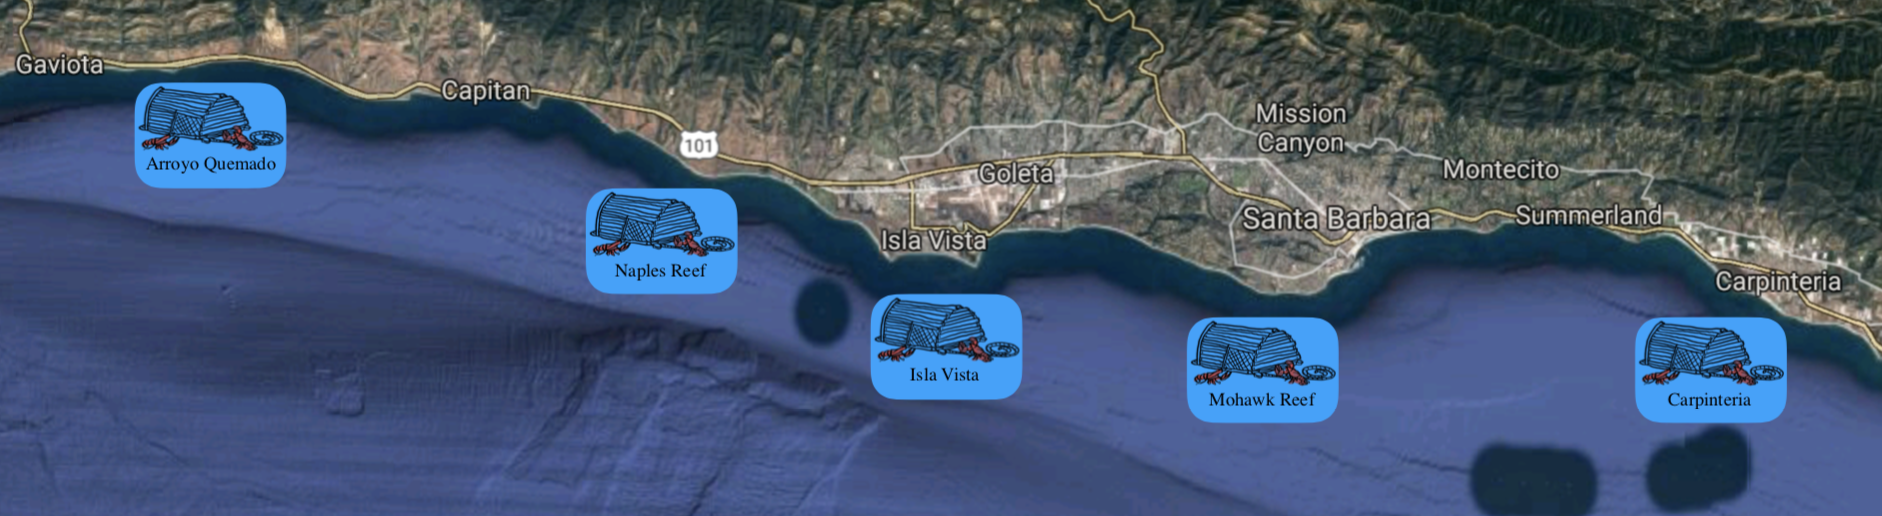
\includegraphics{lobster_map.png}
\caption{\textbf{Figure 1.} Map of locations from which data on Spiny
Lobsters was collected}
\end{figure}

Lobster abundance (measured by counts of individuals) fishing pressure
(measured by number of trap buoys) and lobster size (measured by mean
carapace length) were analyzed to determine trends and significant
differences across the 5 locations. The state of California's South
Coast Supplemental Fishing Report on Spiny Lobster was used to compare
impacts of fishing pressure in MPA and non-MPA locations before and
after their implementation in 2012. Data analysis and visualizations
were performed in R-Studio statistical software (v. 1.1.456), Microsoft
Word (v. 16.18), and Preview (v. 10.1).

\subsection{Results and Discussion}\label{results-and-discussion}

\paragraph{\texorpdfstring{\emph{Trends in Lobster Abundance and Fishing
Pressure between 2012 and
2017}}{Trends in Lobster Abundance and Fishing Pressure between 2012 and 2017}}\label{trends-in-lobster-abundance-and-fishing-pressure-between-2012-and-2017}

Trends in lobster abundance were compared against trends in fishing
pressure and appear to be inversely related. When fishing pressure
decreased, lobster abundance increased. This is reasonable to assume
given fishing by its very nature removes individuals from the
populations studied and therefore decreases measurements of abundance.
The most notable differences were observed at Carpinteria and Isla
Vista. This can be attributed to a 37.5\% decrease in fishing pressure
at both locations from 2016-2017 which allowed populations to more than
triple.

\begin{figure}

{\centering 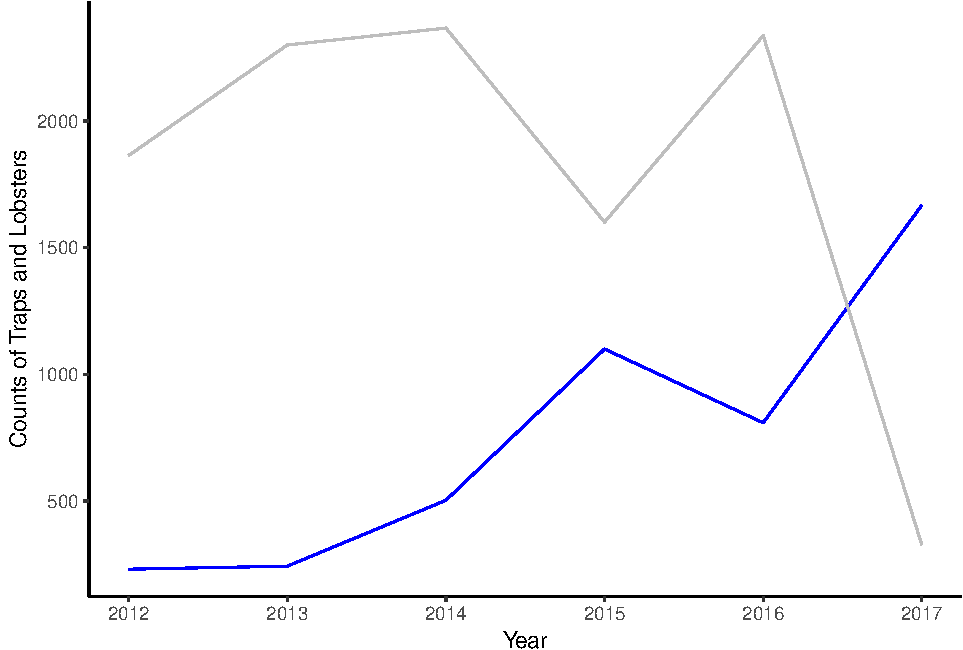
\includegraphics{ESM206_Assignment4_files/figure-latex/unnamed-chunk-3-1} 

}

\caption{**Figure 2. Impact of Fishing Pressure on Lobster abundance** Blue lines indicate populations abundance in number of Spiny Lobsters (Panulirus Interruptus) and grey lines represent fishing pressure as measured by number of fishing trap floats counted. Results are from years 2012 through 2017.}\label{fig:unnamed-chunk-3}
\end{figure}

\paragraph{\texorpdfstring{\emph{Trends in Mean Lobster
Size}}{Trends in Mean Lobster Size}}\label{trends-in-mean-lobster-size}

Mean carapace length (mm) of Spiny Lobsters differed significantly
accross the 5 sites studied for the year 2017 (one-way ANOVA, F(4, 1663)
= 3.42, \emph{p} = 0.009, \(\alpha\) = 0.05). Post-hoc analysis with
Tukey's HSD (\(\alpha\) = 0.05) revealed that the Naples location
differed significantly with Carpinteria and Isla Vista (pairwise
\emph{p} = 0.023, and pairwise \emph{p} = 0.004, respectively). This is
consistent with the marked decrease in fishing pressure in Carpinteria
and Isla Vista compared to Naples where population abundance and fishing
pressure remained relatively flat. The goal of supporting population
growth by limiting fishing appears to be supported by this data but
further analysis is required to determine how such a difference in
individual lobster size could grow while outside pressures remained
relatively constant.

\begin{figure}

{\centering 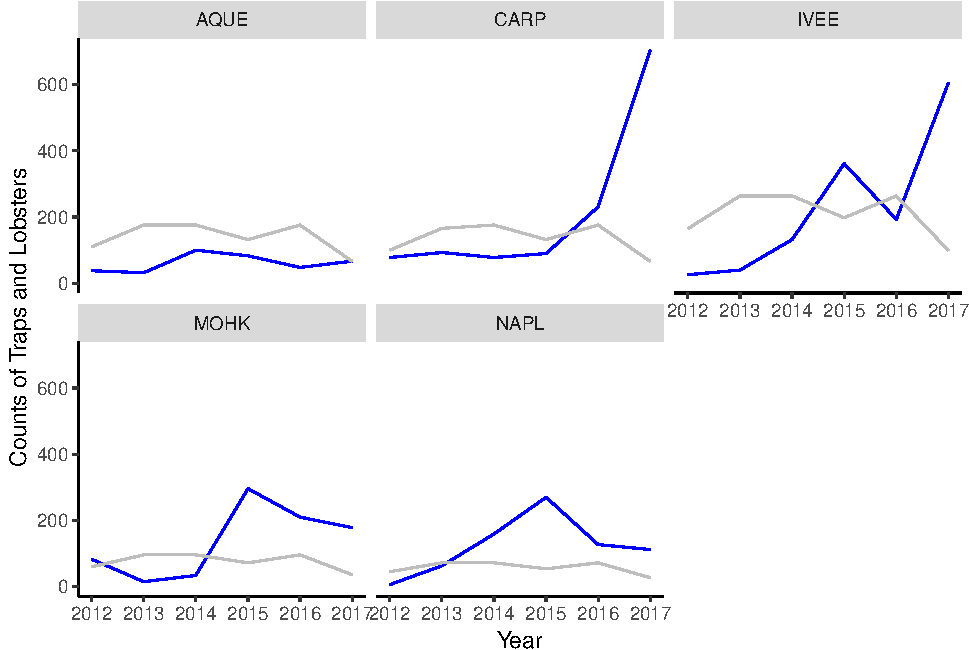
\includegraphics{ESM206_Assignment4_files/figure-latex/unnamed-chunk-4-1} 

}

\caption{**Figure 3. Mean Lobster Size by Location** Observations of mean Spiny Lobster size as measured by carapace length (millimeters) accross all 5 locations studied for the year 2017. Lower and upper boundaries of boxes represent 25th and 75th percentiles, respectively. Whiskers represented are 1.5x the interquartile range. Points indicate outliers. }\label{fig:unnamed-chunk-4}
\end{figure}

Citations

\(^1\)Barsky, K \& Ryan, C., 2003. California Spiny Lobster. Annual
Status of the Fisheries Report.\\
4: 2-12. California Department of Fish and Game.

\(^2\)California Spiny Lobster: Fishing and Life History Information.
California Department of Fish and Wildlife. Ver. 2: 09.18
\url{https://nrm.dfg.ca.gov/FileHandler.ashx?DocumentID=36321\&inline}

\(^3\)Frimodig, A. \& Buck, T., 2017. South Coast Fishery Spotlight:
California Spiny Lobster. State of the California South Coast
Supplemental Report: California Spiny Lobster. 1-6. California
Department of Fish and Wildlife.

\(^4\)NOAA's MPA Inventory, 2018. Data Viewer. National Ocean Service.
\url{https://marineprotectedareas.noaa.gov/dataanalysis/mpainventory/mpaviewer/}

\(^5\)Reed, D. . 2017. SBC LTER: Reef: Abundance, size and fishing
effort for California Spiny Lobster (Panulirus interruptus), ongoing
since 2012. Santa Barbara Coastal Long Term Ecological Research Project.
\url{doi:10.6073/pasta/81ce20b29614ec99d85d54907eaa3e8e}

\(^6\)Research Overview. Santa Barbara Coastal Long Term Ecological
Research. \url{http://sbc.lternet.edu//research/index.html}

\(^7\)Shaw, W. N. 1986. Species profiles: Life Histories and
Environmental Requirements of Coastal Fishes and Invertebrates (Pacific
Southwest)--Spiny Lobster. U.S. Fish Wildlife Serv. Biol.
Rep.~82(11.47). U.S. Army Corps of Engineers, TR EL-82-4. 10 pp.


\end{document}
